\documentclass[10pt]{beamer}

\usepackage{hyperref}
\hypersetup{
    colorlinks=true,
    linkcolor=black,
    filecolor=black,
    urlcolor=blue,
    citecolor=black
}


% Add these packages in the preamble
\usepackage{listings}
\usepackage{xcolor}

% Add this styling configuration
\lstdefinestyle{mystyle}{
    backgroundcolor=\color{gray!10},
    basicstyle=\ttfamily\small,
    breakatwhitespace=false,
    breaklines=true,
    captionpos=b,
    commentstyle=\color{green!60!black},
    keywordstyle=\color{blue},
    stringstyle=\color{red},
    showspaces=false,
    showstringspaces=false,
    showtabs=false,
    tabsize=2,
    frame=single
}
\lstset{style=mystyle}




\usepackage{verbatim}
\usetheme[progressbar=foot]{metropolis}
\usepackage{appendixnumberbeamer}

\usepackage{booktabs}
\usepackage[scale=2]{ccicons}

\usepackage{pgfplots}
\usepgfplotslibrary{dateplot}

\usepackage{xspace}
\usepackage{xcolor}

\usepackage{pifont}
\newcommand{\cmark}{\textcolor{green!70!black}{\ding{51}}} % check mark
\newcommand{\xmark}{\textcolor{red}{\ding{55}}}             % cross mark

\DeclareMathOperator{\stdev}{stdev}
\DeclareMathOperator{\var}{var}
\DeclareMathOperator{\cov}{cov}
\DeclareMathOperator{\corr}{corr}
\DeclareMathOperator{\prob}{prob}
\DeclareMathOperator{\n}{n}
\DeclareMathOperator{\N}{N}
\DeclareMathOperator{\Cov}{Cov}

\newcommand{\D}{\mathrm{d}}
\newcommand{\E}{\mathrm{e}}
\newcommand{\mye}{\ensuremath{\mathsf{E}}}
\newcommand{\myreal}{\ensuremath{\mathbb{R}}}

\setbeamertemplate{frame footer}{MGMT 675}


\setbeamertemplate{title page}{
  \begin{centering}
    \begin{beamercolorbox}[sep=8pt,center]{title}
      \usebeamerfont{title}\inserttitle\par%
      \ifx\insertsubtitle\@empty%
      \else%
        \vskip0.25em%
        {\usebeamerfont{subtitle}\usebeamercolor[fg]{subtitle}\insertsubtitle\par}%
      \fi%     
    \end{beamercolorbox}%
    \vfill
    \begin{beamercolorbox}[sep=8pt,center]{date}
      \usebeamerfont{date}\insertdate
    \end{beamercolorbox}
    \vskip0.5em
    {\usebeamercolor[fg]{titlegraphic}\inserttitlegraphic\par}
  \end{centering}
}


\title{Quantitative Equity Investing}
\subtitle{MGMT 675: AI-Assisted Financial Analysis}
\titlegraphic{
\includegraphics[height=1cm]{../docs/RiceBusiness-transparent-logo-sm.png}}
\date{}
\begin{document}

\begin{frame}[plain]
\titlepage
\end{frame}

\begin{frame}{Outline}
    Motivation: Can we profitably trade on quantitative signals?
    \vspace{1em}
    \begin{enumerate}
    \item Example dataset
    \item Returns of portfolios formed by sorting on characteristics
     \item Regressing returns on characteristics at each date
\item Training a model on past data and sorting on its predictions
    \end{enumerate}
\end{frame}

\section{1. Example Data: stocks.csv}

\begin{frame}[fragile]
\begin{itemize}
    \item Weekly data on stock characteristics, prices, and returns from 2021 to present
    \item Roughly top half of Russell 2000
    \begin{itemize}
    \item Sort on marketcap each week.  
    \item Keep stocks 1,001 through 2,000.  
    \end{itemize}
    \item All items are as of the end-of-week market close except \verb!ret!
    \item \verb!ret! is the return from close of the date shown through close of the following week
    \item Idea is that we trade at each Friday close, holding portfolio until the following Friday close
    \item Original daily data comes from \href{https://www.nasdaq.com/solutions/data/nasdaq-data-link}{Nasdaq Data Link}, specifically \href{https://data.nasdaq.com/databases/SFA}{Sharadar Equity Bundle}
\end{itemize}
\end{frame}

\begin{frame}[fragile]\frametitle{Variables}
\begin{itemize}
        \item \verb!open!, \verb!high!, \verb!low! are for the week
        \item \verb!volume! is average daily volume for the week
        \item \verb!closeunadj! is split but not dividend-adjusted close for the week
        \item \verb!closeadj! is split and dividend-adjusted close for the week
        \item \verb!pb!, \verb!pe!, \verb!ps! are price to book, earnings, and sales
        \item \verb!evebit!, \verb!evebitda! are enterprise value to EBIT and EBITDA
        \item \verb!lag1! is the return over the week ending on the date shown
        \item \verb!lag4! is the return over the prior 4 weeks including the week ending on the date shown, etc.
        \item \verb!rsi! is the \href{https://en.wikipedia.org/wiki/Relative_strength_index}{Relative Strength Index}
\end{itemize}
\end{frame}

\section{2. Sorting}

\begin{frame}[fragile]\frametitle{Method}
\begin{itemize}
\item Sort stocks on some characteristic into quintiles (for example) \alert{at each date}.
\item Compute the average value of \verb!ret! in each quintile at each date.  This is the return of an equally weighted portfolio of the stocks in that group (weights $=1/n$).
\item Compare the returns over time of the quintile portfolios: mean, standard deviation, Sharpe ratio, (and alphas).
\item Also look at the $5-1$ or $1-5$ portfolio: long one extreme quintile and short the other extreme.
\item Annualize means, std devs, Sharpe ratios by multiplying by 52, $\sqrt{52}$, and $\sqrt{52}$ respectively.
\end{itemize}
\end{frame}

\begin{frame}{Sample Questions to Answer}
\begin{itemize}
    \item Do stocks with higher returns last week (or last month or \ldots) tend to have higher returns in the future, or should you be a contrarian?  I.e., is there momentum or reversal on average?
    \item Is there a value effect in the data?
\end{itemize}
\end{frame}

\section{3. Regressions}

\begin{frame}[fragile]\frametitle{Regression Example}
    \begin{itemize}
    \item At a given date, run a regression over the 1,000 stock observations with $y=$ \verb!ret! and $x_1, \ldots, x_n = $ some characteristics.
    \item Example: April 4, 2025.  Characteristics = \verb!pb!, \verb!lag52!, \verb!lag4!, \verb!rsi!.
   
    \vspace{1em}
    \begin{center}
        \begin{tabular}{lcccccc}
        \toprule
                       & \textbf{coef} & \textbf{std err} & \textbf{t} & \textbf{P$> |$t$|$} & \textbf{[0.025} & \textbf{0.975]}  \\
        \midrule
        \textbf{const} &      -3.001  &        1.390     &    -2.159  &         0.031        &       -5.729    &       -0.273     \\
        \textbf{pb}    &       0.042  &        0.016     &     2.631  &         0.009        &        0.011    &        0.074     \\
        \textbf{lag52} &       0.019  &        0.004     &     4.912  &         0.000        &        0.012    &        0.027     \\
        \textbf{lag4}  &      -0.124  &        0.028     &    -4.406  &         0.000        &       -0.179    &       -0.069     \\
        \textbf{rsi}   &       0.077  &        0.034     &     2.266  &         0.024        &        0.010    &        0.144     \\
        \bottomrule
        \end{tabular}
        \end{center}
        \vspace{1em}
    \item Interpretation example: if stocks A and B have past-4-week returns of 8\% and 9\% respectively, and have the same values for the other variables, then we would expect the return of stock B in the next week to be 12.4 basis points lower than the return of stock A.
    \end{itemize}
    \end{frame}

\begin{frame}[fragile]\frametitle{Regression at Every Date}
\begin{itemize}
\item To determine whether stocks with higher \verb!lag4! usually have lower returns, we can run the regression at every date.
\item Collect the regression coefficients at all dates.
\item Is the coefficient on \verb!lag4! negative on average?
\item Is it statistically significant? Instead of checking significance at a single date, consider the series of coefficients as a sample and \alert{run a $t$ test}.
\item Called Fama-MacBeth regressions.
\end{itemize}
\end{frame}


\begin{frame}[fragile]\frametitle{Sample Julius Prompt}
    Ask Julius to run a regression of \verb!ret! on \verb!pb!, \verb!lag52!, \verb!lag4!, and \verb!rsi! at each date.  Collect the slope coefficients across dates and run a t-test on each one.
\vspace{2em}

    Or try this (it will probably work): Ask Julius to run Fama-MacBeth regressions of of \verb!ret! on \verb!pb!, \verb!lag52!, \verb!lag4!, and \verb!rsi! and test for statistical significance.
\end{frame}

\section{4. Train a Model and Trade on It}

\begin{frame}[fragile]\frametitle{Overview}
    \begin{itemize}
    \item At some date, use the \alert{panel} of past data to estimate (= fit = train) a model with $y=$ \verb!ret! and some $x$ variables (characteristics).
    \begin{itemize}
    \item Panel = all stocks at all past dates
    \item A panel is a two-dimensional array of data, one dimension being \verb!ticker! and the other dimension being \verb!date!.
    \end{itemize}
    \item Use the trained model and current characteristics to predict future returns.
    \item Form portfolios based on the predictions -- for example, sort into quintiles.
    \item Can retrain next week with another week of data and use that model to predict for the following week, etc.
    \end{itemize}
\end{frame}

\begin{frame}[fragile]\frametitle{Need to Use Relative Data}
    \begin{itemize}
    \item Below is a plot of the median value of \verb!lag52! over time.
    \item A value of \verb!lag52! of, e.g., 40\% did not mean the same thing in the spring of 2022 as it did in the spring of 2021.
    \end{itemize}
    \begin{center}
    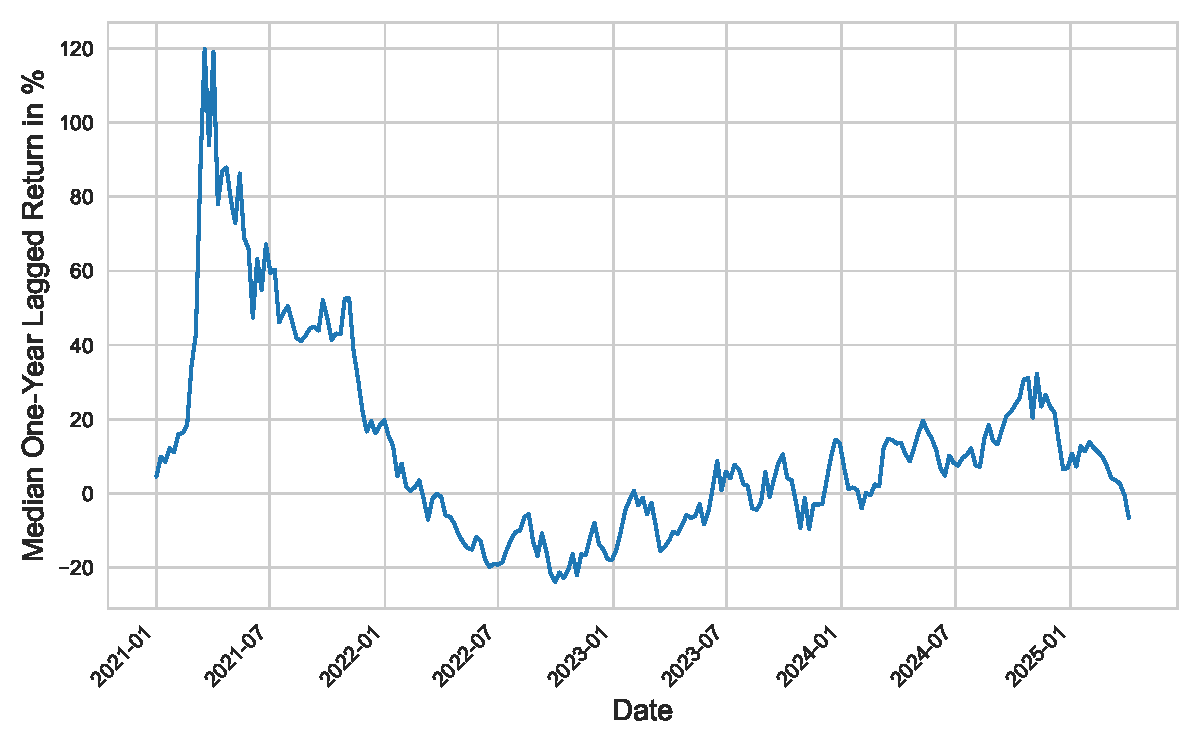
\includegraphics[width=0.8\textwidth]{lagret.pdf}
    \end{center}
     \end{frame}

\begin{frame}[fragile]\frametitle{Standardize at Each Date}
    \begin{itemize}
    \item At each date, standardize each feature to be used in the model by subtracting its mean value at that date and dividing by its standardization at that date.
    \begin{itemize}
    \item This results in each feature at each date having a mean of 0 and a std dev of 1.
    \item Avoids issue of noncomparability across dates and also makes models easier to train.
    \end{itemize}
    \item At each date, standardize \verb!ret! the same way.
    \begin{itemize}
    \item Hard to forecast the market.
    \item So, easier to forecast performance relative to the market (which stocks will beat the market and which won't) than to forecast absolute returns.
    \end{itemize}
\end{itemize}
    \end{frame}

\begin{frame}[fragile]\frametitle{Summary of Method}
\begin{enumerate}
\item Standardize all variables at each date (subtract mean and divide by std dev) -- in the code, you might see StandardScaler used for this.  \alert{Important: define the standardized return to be a new variable, for example stdret.}
\item At a given date (e.g., 2024-01-01), use all data prior to that date to train a model to predict \verb!stdret! from standardized features.
\item Use the model and the same standardized features at 2024-01-01 and all subsequent dates to predict \verb!stdret!.
\item Sort into quintiles at 2024-01-01 and all subsequent dates based on the predictions and compute the mean \verb!ret! in each quintile at each date.  \alert{Important: compute the mean return not the mean standardized return.}
\item Analyze the quintile returns over time and the long-short return $5-1$: mean and Sharpe ratio.  Annualize for easier interpretability.
\end{enumerate}
\end{frame}

\begin{frame}[fragile]\frametitle{Question}
    If you use a multi-layer perceptron and \verb!pb!, \verb!lag52!, \verb!lag4!, and \verb!rsi! as the features, can you use the predictions from a trained model to trade successfully? 
    
    \vspace{1em}
    Julius may default to a network structure that is too simple, for example, 2 hidden layers with 16 and 4 neurons respectively.  You may want to ask for a more complex network, for example, three hidden layers with 64, 64, and 32 neurons respectively.
    \vspace{1em}

    \alert{Caution: Others are already using more sophisticated versions of this, so the market should be mostly efficient.  E.g., \href{https://mgmt675-2024.kerryback.com/assets/Gu_Kelly_Xiu_RFS_2020.pdf}{Gu-Kelly-Xiu (2020)}}
    \vspace{1em}
    
    \alert{Also, we are ignoring the fact that you buy at the ask and sell at the bid, which causes round-trip transactions to be costly.}
\end{frame}
\end{document}

